\def\dt{\,\text{dt}\,}
\chapter{Vorbereitung}
    \section{Fourierreihen und -transformation}
Die Fourier-Analysis findet gerade in der Optik häufig Anwendung. Im Kontext der 
Holografie stellen vor allem Fourierreihen und die Fouriertransformation nützliche
Hilfsmittel dar, weshalb diese zur Vorbereitung näher betrachtet werden sollen.
    \subsection*{Fourierreihenentwicklung}
Die Fourierreihe bietet die Möglichkeit einen großen Teil der periodischen 
Funktionen durch eine Linearkombination von Sinus- und Kosinustermen verschiedener
Frequenzen und Amplituden zu entwickeln.
        \begin{align*}
           f(t) = \sum_{k=0}^\infty a_k \cos(\omega_k \, t) + b_k \sin(\omega_k \, t) 
           \qquad \text{mit  } \omega_k =  \frac{2 \pi k}{T}
        \end{align*}
$T$ sei hierbei die Periodendauer der Funktion. Die \emph{Fourierkoeffizienten} $a_k$
und $b_k$ werden hier beschrieben durch
        \begin{align*}
            a_0 = \frac{1}{T} \int_{-T/2}^{+T/2} f(t) \dt \quad &a_k = \frac{2}{T} \int_{-T/2}^{+T/2} f(t) \cos(\omega_k \, t) \dt \;(k\neq 0)\\
            &b_k = \frac{2}{T} \int_{-T/2}^{+T/2} f(t) \sin()\omega_k \, t) \dt
        \end{align*}
Dies soll nun an zwei wichtigen Funktionen demonstriert werden.
            \subsubsection*{Rechtecksfunktion}
        \begin{wrapfigure}{r}{0.45\textwidth}
            \vspace{10pt}
            \centering
            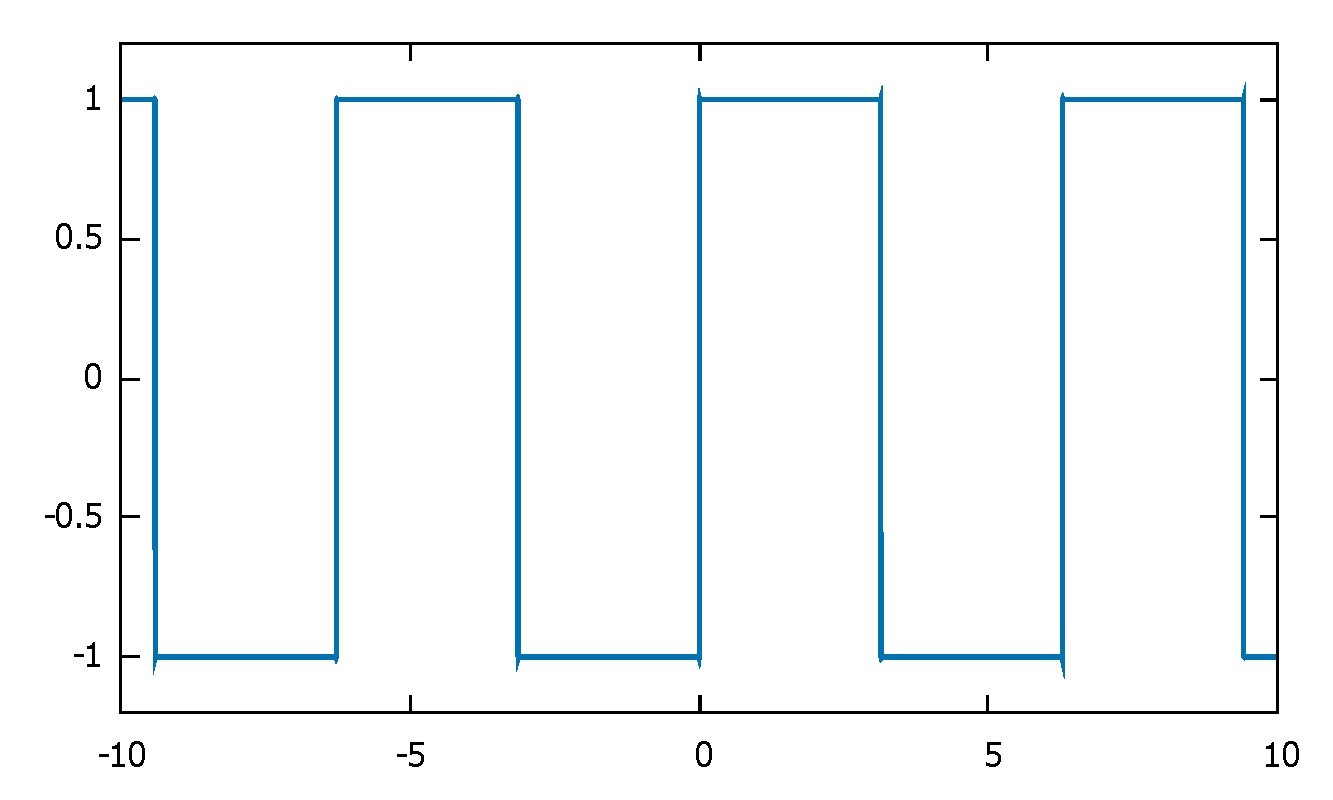
\includegraphics[width=0.35\textwidth]{Abb/rechteck.pdf}
            \caption{Rechtecksfunktion}
            \vspace{10pt}
        \end{wrapfigure}
Die Rechtecksfunktion ist gegeben durch
        \begin{align*}
            f(t) = \begin{cases}
                -1 & \text{für } -1 < t < 0 \\
                 1 & \text{für }  0 < t < 1
            \end{cases}   
        \end{align*}
mit periodischer Fortsetzung.\\
Um nun die Fourierreihendarstellung nutzen zu können, müssen zuerst die Koeffizienten
errechnet werden. Für $T=2$ ergibt sich:
        \begin{itemize}
            \item da die Rechtecksfunktion eine ungerade Funktion ist gilt $a_k = 0$
            \item für die $b_k$ gilt
                \begin{align*}
                   b_k &=\frac{2}{2} \int_{-1}^{1} f(t) \sin(\pi k t ) \dt = 
                   \int_{-1}^{0} - \sin(\omega_k t) \dt 
                   + \int_0^1 \sin(\omega_k t ) \dt \\
                   &= \frac{1}{\pi k} \left[
                       \left(1 - \cos
                        \left(-\frac{\pi k}{2}
                        \right)
                       \right)
                     + \left(-\cos
                        \left( \frac{\pi k}{2}
                        \right) + 1
                       \right)
                    \right]
                    = \frac{2}{\pi k} \left( 1 + \cos(\pi k)\right)
                \end{align*}
            \end{itemize}
Somit erhalten wir für die Fourierreihenentwicklung der Rechtecksfunktion
                \begin{align*}
                   f(t) = \sum_{k=0}^\infty \frac{2}{\pi k} (1 + \cos(\pi k)) 
                   \sin(\pi k t) 
                \end{align*}
                \begin{figure}[htb]
                   \centering
                   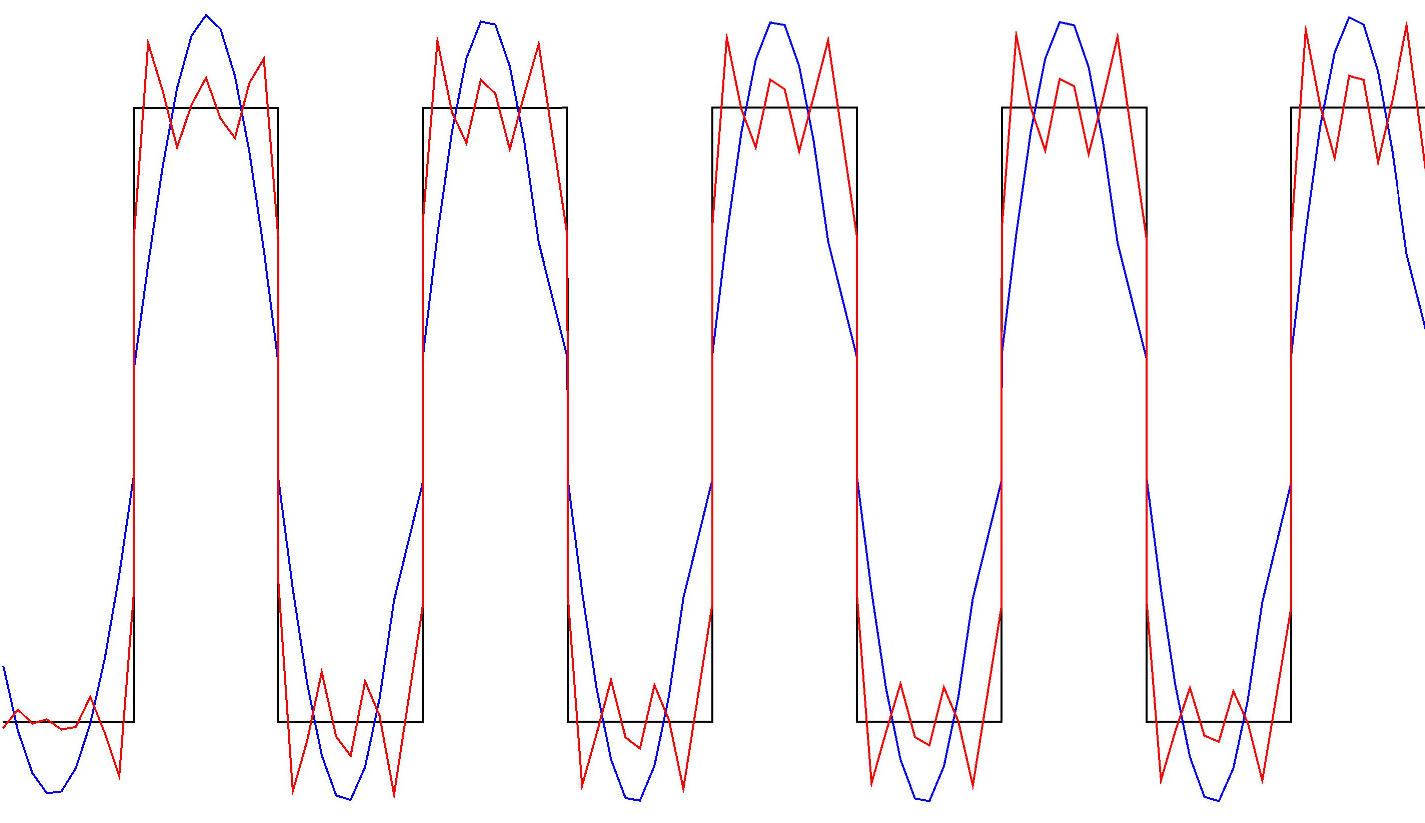
\includegraphics[width=0.8\textwidth]{Abb/rechteck_fit.pdf} 
                   \caption{Die Rechtecksfunktion und die Reihenentwicklung für 1 und 2}
                \end{figure}

                    \subsubsection*{Dreiecksfunktion}
Die Dreiecksfunktion ist gegeben durch
                \begin{align*}
                   g(t) = \begin{cases}
                    -2(x+1) & \text{für } -1   < t < -0,5 \\
                    2x      & \text{für } -0,5 < t <  0,5 \\
                    2(x+1)  & \text{für } 0,5  < t <  1
                        \end{cases}
                \end{align*}